\documentclass{standalone}
\usepackage[utf8]{inputenc}
\usepackage{pgfplots}
\DeclareUnicodeCharacter{2212}{−}
\usepgfplotslibrary{groupplots}
\usepgfplotslibrary{dateplot}
\usetikzlibrary{patterns}
\usetikzlibrary{shapes.arrows}
\pgfplotsset{compat=newest}
\begin{document}
% This file was created by tikzplotlib v0.9.1.
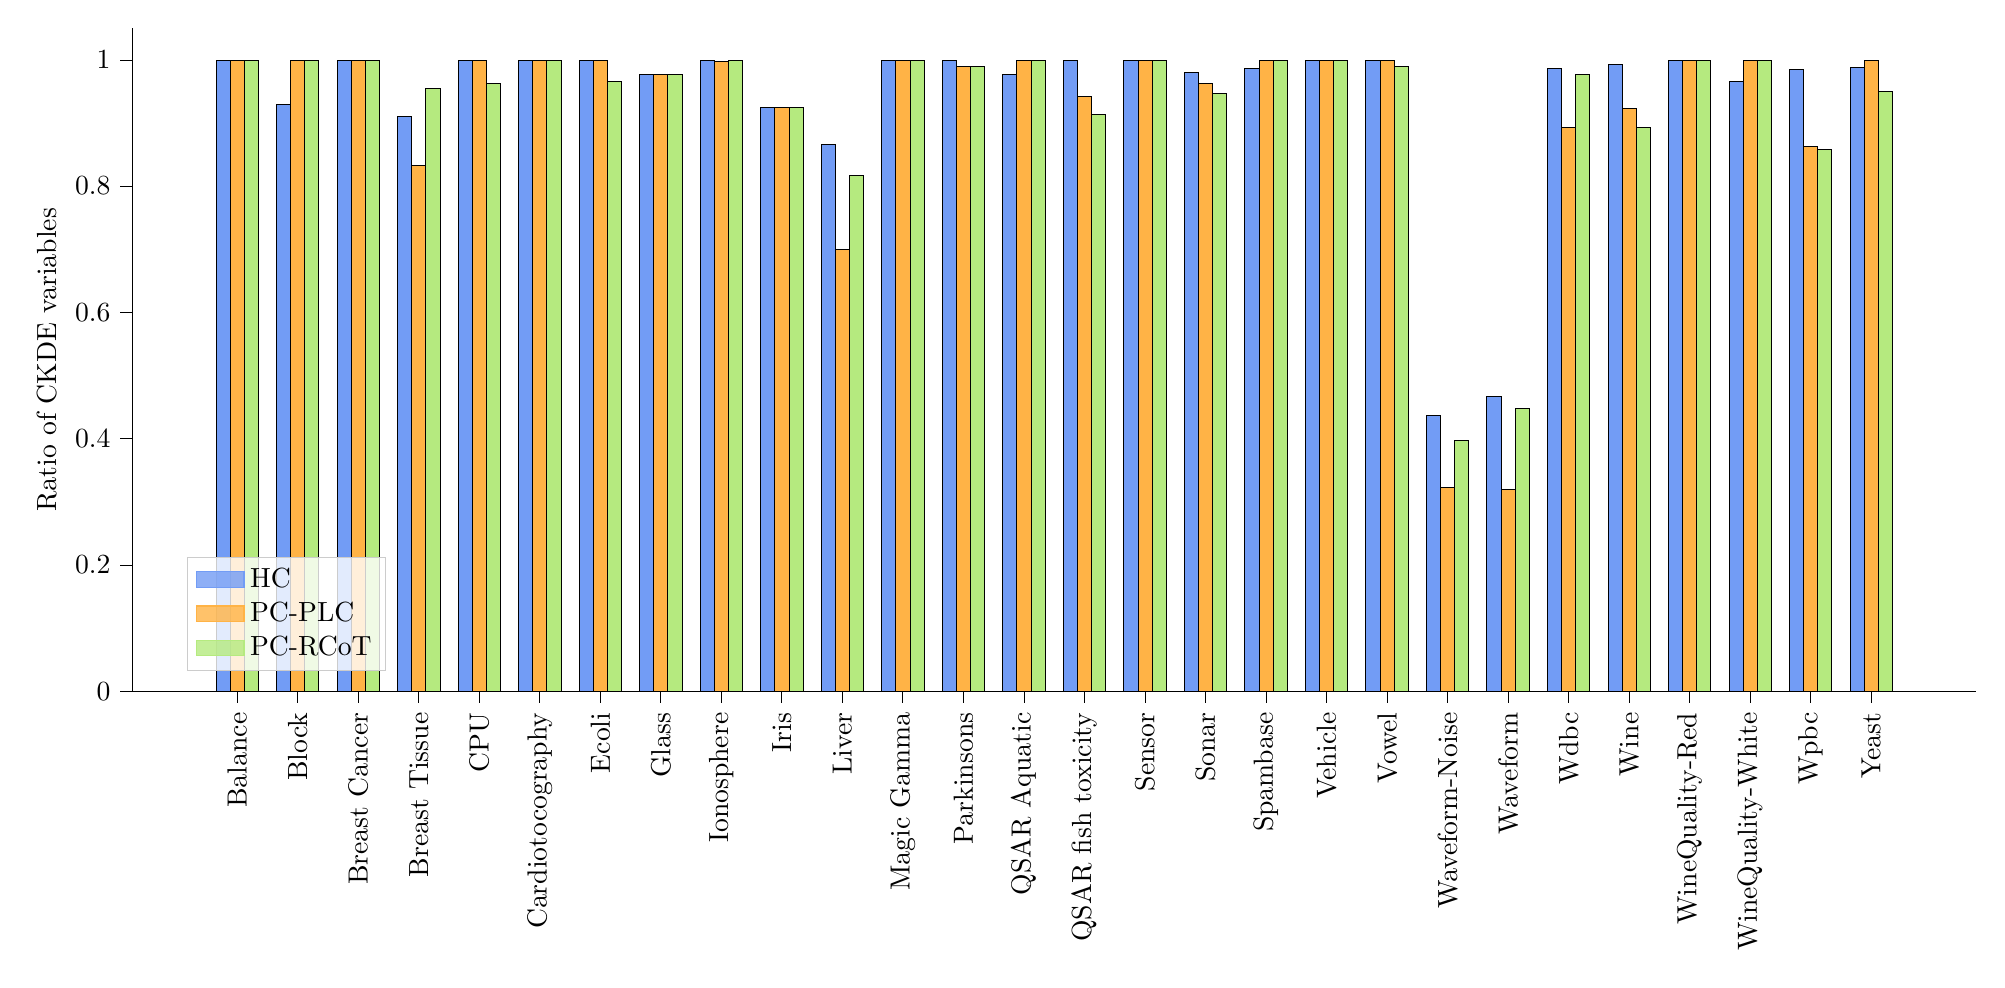
\begin{tikzpicture}

\definecolor{color0}{rgb}{0.447058823529412,0.611764705882353,0.96078431372549}
\definecolor{color1}{rgb}{1,0.701960784313725,0.274509803921569}
\definecolor{color2}{rgb}{0.709803921568627,0.917647058823529,0.498039215686275}

\begin{axis}[
height=10cm,
legend cell align={left},
legend style={fill opacity=0.8, draw opacity=1, text opacity=1, at={(0.03,0.97)}, anchor=north west, draw=white!80!black},
tick align=outside,
tick pos=left,
width=25cm,
x grid style={white!69.0196078431373!black},
xmin=-1.385, xmax=29.085,
xtick style={color=black},
xtick={0.35,1.35,2.35,3.35,4.35,5.35,6.35,7.35,8.35,9.35,10.35,11.35,12.35,13.35,14.35,15.35,16.35,17.35,18.35,19.35,20.35,21.35,22.35,23.35,24.35,25.35,26.35,27.35},
xticklabel style = {rotate=90.0},
xticklabels={Balance,Block,Breast Cancer,Breast Tissue,CPU,Cardiotocography,Ecoli,Glass,Ionosphere,Iris,Liver,Magic Gamma,Parkinsons,QSAR Aquatic,QSAR fish toxicity,Sensor,Sonar,Spambase,Vehicle,Vowel,Waveform-Noise,Waveform,Wdbc,Wine,WineQuality-Red,WineQuality-White,Wpbc,Yeast},
y grid style={white!69.0196078431373!black},
ylabel={Ratio of CKDE variables},
ymin=0, ymax=1.05,
ytick style={color=black},
legend pos = south west,
axis x line*=bottom,
axis y line*=left
]
\draw[draw=black,fill=color0,very thin] (axis cs:0,0) rectangle (axis cs:0.233333333333333,1);
\draw[draw=black,fill=color0,very thin] (axis cs:1,0) rectangle (axis cs:1.23333333333333,0.93);
\draw[draw=black,fill=color0,very thin] (axis cs:2,0) rectangle (axis cs:2.23333333333333,1);
\draw[draw=black,fill=color0,very thin] (axis cs:3,0) rectangle (axis cs:3.23333333333333,0.911111111111111);
\draw[draw=black,fill=color0,very thin] (axis cs:4,0) rectangle (axis cs:4.23333333333333,1);
\draw[draw=black,fill=color0,very thin] (axis cs:5,0) rectangle (axis cs:5.23333333333333,1);
\draw[draw=black,fill=color0,very thin] (axis cs:6,0) rectangle (axis cs:6.23333333333333,1);
\draw[draw=black,fill=color0,very thin] (axis cs:7,0) rectangle (axis cs:7.23333333333333,0.977777777777778);
\draw[draw=black,fill=color0,very thin] (axis cs:8,0) rectangle (axis cs:8.23333333333333,1);
\draw[draw=black,fill=color0,very thin] (axis cs:9,0) rectangle (axis cs:9.23333333333333,0.925);
\draw[draw=black,fill=color0,very thin] (axis cs:10,0) rectangle (axis cs:10.2333333333333,0.866666666666667);
\draw[draw=black,fill=color0,very thin] (axis cs:11,0) rectangle (axis cs:11.2333333333333,1);
\draw[draw=black,fill=color0,very thin] (axis cs:12,0) rectangle (axis cs:12.2333333333333,1);
\draw[draw=black,fill=color0,very thin] (axis cs:13,0) rectangle (axis cs:13.2333333333333,0.977777777777778);
\draw[draw=black,fill=color0,very thin] (axis cs:14,0) rectangle (axis cs:14.2333333333333,1);
\draw[draw=black,fill=color0,very thin] (axis cs:15,0) rectangle (axis cs:15.2333333333333,1);
\draw[draw=black,fill=color0,very thin] (axis cs:16,0) rectangle (axis cs:16.2333333333333,0.98);
\draw[draw=black,fill=color0,very thin] (axis cs:17,0) rectangle (axis cs:17.2333333333333,0.985964912280702);
\draw[draw=black,fill=color0,very thin] (axis cs:18,0) rectangle (axis cs:18.2333333333333,1);
\draw[draw=black,fill=color0,very thin] (axis cs:19,0) rectangle (axis cs:19.2333333333333,1);
\draw[draw=black,fill=color0,very thin] (axis cs:20,0) rectangle (axis cs:20.2333333333333,0.4375);
\draw[draw=black,fill=color0,very thin] (axis cs:21,0) rectangle (axis cs:21.2333333333333,0.466666666666667);
\draw[draw=black,fill=color0,very thin] (axis cs:22,0) rectangle (axis cs:22.2333333333333,0.986666666666667);
\draw[draw=black,fill=color0,very thin] (axis cs:23,0) rectangle (axis cs:23.2333333333333,0.992307692307692);
\draw[draw=black,fill=color0,very thin] (axis cs:24,0) rectangle (axis cs:24.2333333333333,1);
\draw[draw=black,fill=color0,very thin] (axis cs:25,0) rectangle (axis cs:25.2333333333333,0.966666666666667);
\draw[draw=black,fill=color0,very thin] (axis cs:26,0) rectangle (axis cs:26.2333333333333,0.984848484848485);
\draw[draw=black,fill=color0,very thin] (axis cs:27,0) rectangle (axis cs:27.2333333333333,0.9875);
\draw[draw=black,fill=color1,very thin] (axis cs:0.233333333333333,0) rectangle (axis cs:0.466666666666667,1);
\draw[draw=black,fill=color1,very thin] (axis cs:1.23333333333333,0) rectangle (axis cs:1.46666666666667,1);
\draw[draw=black,fill=color1,very thin] (axis cs:2.23333333333333,0) rectangle (axis cs:2.46666666666667,1);
\draw[draw=black,fill=color1,very thin] (axis cs:3.23333333333333,0) rectangle (axis cs:3.46666666666667,0.833333333333333);
\draw[draw=black,fill=color1,very thin] (axis cs:4.23333333333333,0) rectangle (axis cs:4.46666666666667,1);
\draw[draw=black,fill=color1,very thin] (axis cs:5.23333333333333,0) rectangle (axis cs:5.46666666666667,1);
\draw[draw=black,fill=color1,very thin] (axis cs:6.23333333333333,0) rectangle (axis cs:6.46666666666667,1);
\draw[draw=black,fill=color1,very thin] (axis cs:7.23333333333333,0) rectangle (axis cs:7.46666666666667,0.977777777777778);
\draw[draw=black,fill=color1,very thin] (axis cs:8.23333333333333,0) rectangle (axis cs:8.46666666666667,0.996969696969697);
\draw[draw=black,fill=color1,very thin] (axis cs:9.23333333333333,0) rectangle (axis cs:9.46666666666667,0.925);
\draw[draw=black,fill=color1,very thin] (axis cs:10.2333333333333,0) rectangle (axis cs:10.4666666666667,0.7);
\draw[draw=black,fill=color1,very thin] (axis cs:11.2333333333333,0) rectangle (axis cs:11.4666666666667,1);
\draw[draw=black,fill=color1,very thin] (axis cs:12.2333333333333,0) rectangle (axis cs:12.4666666666667,0.990476190476191);
\draw[draw=black,fill=color1,very thin] (axis cs:13.2333333333333,0) rectangle (axis cs:13.4666666666667,1);
\draw[draw=black,fill=color1,very thin] (axis cs:14.2333333333333,0) rectangle (axis cs:14.4666666666667,0.942857142857143);
\draw[draw=black,fill=color1,very thin] (axis cs:15.2333333333333,0) rectangle (axis cs:15.4666666666667,1);
\draw[draw=black,fill=color1,very thin] (axis cs:16.2333333333333,0) rectangle (axis cs:16.4666666666667,0.963333333333333);
\draw[draw=black,fill=color1,very thin] (axis cs:17.2333333333333,0) rectangle (axis cs:17.4666666666667,1);
\draw[draw=black,fill=color1,very thin] (axis cs:18.2333333333333,0) rectangle (axis cs:18.4666666666667,1);
\draw[draw=black,fill=color1,very thin] (axis cs:19.2333333333333,0) rectangle (axis cs:19.4666666666667,1);
\draw[draw=black,fill=color1,very thin] (axis cs:20.2333333333333,0) rectangle (axis cs:20.4666666666667,0.3225);
\draw[draw=black,fill=color1,very thin] (axis cs:21.2333333333333,0) rectangle (axis cs:21.4666666666667,0.319047619047619);
\draw[draw=black,fill=color1,very thin] (axis cs:22.2333333333333,0) rectangle (axis cs:22.4666666666667,0.893333333333333);
\draw[draw=black,fill=color1,very thin] (axis cs:23.2333333333333,0) rectangle (axis cs:23.4666666666667,0.923076923076923);
\draw[draw=black,fill=color1,very thin] (axis cs:24.2333333333333,0) rectangle (axis cs:24.4666666666667,1);
\draw[draw=black,fill=color1,very thin] (axis cs:25.2333333333333,0) rectangle (axis cs:25.4666666666667,1);
\draw[draw=black,fill=color1,very thin] (axis cs:26.2333333333333,0) rectangle (axis cs:26.4666666666667,0.863636363636364);
\draw[draw=black,fill=color1,very thin] (axis cs:27.2333333333333,0) rectangle (axis cs:27.4666666666667,1);
\draw[draw=black,fill=color2,very thin] (axis cs:0.466666666666667,0) rectangle (axis cs:0.7,1);
\draw[draw=black,fill=color2,very thin] (axis cs:1.46666666666667,0) rectangle (axis cs:1.7,1);
\draw[draw=black,fill=color2,very thin] (axis cs:2.46666666666667,0) rectangle (axis cs:2.7,1);
\draw[draw=black,fill=color2,very thin] (axis cs:3.46666666666667,0) rectangle (axis cs:3.7,0.955555555555555);
\draw[draw=black,fill=color2,very thin] (axis cs:4.46666666666667,0) rectangle (axis cs:4.7,0.9625);
\draw[draw=black,fill=color2,very thin] (axis cs:5.46666666666667,0) rectangle (axis cs:5.7,1);
\draw[draw=black,fill=color2,very thin] (axis cs:6.46666666666667,0) rectangle (axis cs:6.7,0.966666666666667);
\draw[draw=black,fill=color2,very thin] (axis cs:7.46666666666667,0) rectangle (axis cs:7.7,0.977777777777778);
\draw[draw=black,fill=color2,very thin] (axis cs:8.46666666666667,0) rectangle (axis cs:8.7,1);
\draw[draw=black,fill=color2,very thin] (axis cs:9.46666666666667,0) rectangle (axis cs:9.7,0.925);
\draw[draw=black,fill=color2,very thin] (axis cs:10.4666666666667,0) rectangle (axis cs:10.7,0.816666666666667);
\draw[draw=black,fill=color2,very thin] (axis cs:11.4666666666667,0) rectangle (axis cs:11.7,1);
\draw[draw=black,fill=color2,very thin] (axis cs:12.4666666666667,0) rectangle (axis cs:12.7,0.990476190476191);
\draw[draw=black,fill=color2,very thin] (axis cs:13.4666666666667,0) rectangle (axis cs:13.7,1);
\draw[draw=black,fill=color2,very thin] (axis cs:14.4666666666667,0) rectangle (axis cs:14.7,0.914285714285714);
\draw[draw=black,fill=color2,very thin] (axis cs:15.4666666666667,0) rectangle (axis cs:15.7,1);
\draw[draw=black,fill=color2,very thin] (axis cs:16.4666666666667,0) rectangle (axis cs:16.7,0.946666666666667);
\draw[draw=black,fill=color2,very thin] (axis cs:17.4666666666667,0) rectangle (axis cs:17.7,1);
\draw[draw=black,fill=color2,very thin] (axis cs:18.4666666666667,0) rectangle (axis cs:18.7,1);
\draw[draw=black,fill=color2,very thin] (axis cs:19.4666666666667,0) rectangle (axis cs:19.7,0.99);
\draw[draw=black,fill=color2,very thin] (axis cs:20.4666666666667,0) rectangle (axis cs:20.7,0.3975);
\draw[draw=black,fill=color2,very thin] (axis cs:21.4666666666667,0) rectangle (axis cs:21.7,0.447619047619048);
\draw[draw=black,fill=color2,very thin] (axis cs:22.4666666666667,0) rectangle (axis cs:22.7,0.976666666666667);
\draw[draw=black,fill=color2,very thin] (axis cs:23.4666666666667,0) rectangle (axis cs:23.7,0.892307692307692);
\draw[draw=black,fill=color2,very thin] (axis cs:24.4666666666667,0) rectangle (axis cs:24.7,1);
\draw[draw=black,fill=color2,very thin] (axis cs:25.4666666666667,0) rectangle (axis cs:25.7,1);
\draw[draw=black,fill=color2,very thin] (axis cs:26.4666666666667,0) rectangle (axis cs:26.7,0.857575757575758);
\draw[draw=black,fill=color2,very thin] (axis cs:27.4666666666667,0) rectangle (axis cs:27.7,0.95);

\addlegendimage{area legend,fill=color0, color=color0}
\addlegendimage{area legend,fill=color1, color=color1}
\addlegendimage{area legend,fill=color2, color=color2}
\legend{HC, PC-PLC, PC-RCoT}
\end{axis}

\end{tikzpicture}

\end{document}
